\documentclass{article}
\usepackage[T1]{fontenc}  
\usepackage[utf8]{inputenc}  
\usepackage[vietnamese]{babel}  
\usepackage{graphicx}  
\usepackage{hyperref}
\usepackage[utf8]{vietnam}
\usepackage{amsmath}
\usepackage{enumitem}
\usepackage{tikz}
\usepackage{tabularx}
\usepackage[a4paper, left=1.5in, right=1in, top=1in, bottom=1in]{geometry} % Điều chỉnh lề
\usepackage{setspace} % Để điều chỉnh giãn dòng
\usepackage{indentfirst} % Thụt lề đầu dòng
% \usepackage[fontsize=13pt]{scrextend} 

% Định dạng đoạn văn
\setlength{\parindent}{1.27cm} % Thụt lề đầu dòng 1.27cm
\setlength{\parskip}{6pt} % Khoảng cách giữa các đoạn
\onehalfspacing % Giãn dòng 1.5


\begin{document}

\begin{titlepage}
    \begin{tikzpicture}[remember picture, overlay]
        % Vẽ khung trang trí gần mép trang
        \draw[thick, rounded corners, draw=blue!50!black] 
            ([shift={(1cm,-1cm)}]current page.north west) 
            rectangle 
            ([shift={(-1cm,1cm)}]current page.south east);
        % Vẽ khung bên trong (tùy chọn)
        \draw[dashed, draw=red!70!black] 
            ([shift={(1.5cm,-1.5cm)}]current page.north west) 
            rectangle 
            ([shift={(-1.5cm,1.5cm)}]current page.south east);
    \end{tikzpicture}

    \vspace*{-1cm} 
    \centering

    % Phần tiêu đề
    {\LARGE \textbf{UỶ BAN NHÂN DÂN THÀNH PHỐ HỒ CHÍ MINH}} \\[0.5cm] % Tạo khoảng cách giữa dòng đầu và dòng sau
    {\Large \textbf{\underline{TRƯỜNG ĐẠI HỌC SÀI GÒN}}} \\[1cm]

    % Chèn logo
    
\includegraphics[width=4cm]{./img/logo.png} \\[1cm]

    % Tiêu đề luận văn
    {\huge \textbf{NHẬN DIỆN BIỂU CẢM KHUÔN MẶT TRONG ĐIỀU KIỆN ÁNH SÁNG YẾU SỬ DỤNG CNN NHẸ KẾT HỢP KỸ THUẬT TĂNG CƯỜNG DỮ LIỆU THÍCH ỨNG}} \\[1.5cm]

    % Mô tả luận văn
    {\Large \textbf{LUẬN VĂN MÔN HỌC NCKH TRONG CNTT}} \\[0.5cm]
    {\Large NGÀNH: CÔNG NGHỆ THÔNG TIN} \\[1cm]

    % Thông tin nhóm sinh viên
    \textbf{Nhóm sinh viên thực hiện: (Nhóm 17)} \\[0.5cm]
    \begin{tabular}{l l}
        \textbf{Họ và tên} & \textbf{MSSV} \\ 
        Văn Tuấn Kiệt & 3122410202 \\ 
        Mai Phúc Lâm & 3122410207 \\ 
        Nguyễn Đức Duy Lâm & 3122410208 \\ 
        Nguyễn Hữu Lộc & 3122410213 \\ 
    \end{tabular}
    \\[1cm]  % Thêm khoảng cách giữa bảng và phần tiếp theo
    % Thông tin giáo viên hướng dẫn
    \textbf{Giáo viên hướng dẫn:} Đỗ Như Tài \\[0.5cm]
    % Ngày tháng
    \textbf{ 05/2025, TP.HCM }
\end{titlepage}

\newpage 
% Áp dụng cỡ chữ 13pt
\begingroup
\fontsize{13pt}{18pt}\selectfont

\begin{center}
    {\LARGE \textbf{ĐỀ CƯƠNG LUẬN VĂN}} \\[1cm]
\end{center}

\section{Lý do chọn đề tài}

Trong thời đại công nghệ số và trí tuệ nhân tạo phát triển mạnh mẽ, các hệ thống nhận diện biểu cảm khuôn mặt (Facial Expression Recognition - FER) ngày càng đóng vai trò quan trọng trong nhiều lĩnh vực như giám sát an ninh, giáo dục thông minh, chăm sóc sức khỏe, và tương tác người - máy. Tuy nhiên, một trong những thách thức lớn mà các hệ thống FER hiện nay gặp phải là điều kiện ánh sáng không ổn định, đặc biệt là ánh sáng yếu – tình huống phổ biến trong môi trường thực tế như ban đêm, nhà thông minh hoặc thiết bị giám sát có cấu hình thấp.

Nhiều nghiên cứu hiện tại đã áp dụng các mô hình học sâu như CNN, GAN hay các phương pháp tiền xử lý hình ảnh phức tạp để cải thiện hiệu suất trong điều kiện ánh sáng yếu. Tuy nhiên, phần lớn các phương pháp này đòi hỏi tài nguyên tính toán cao, khó triển khai trên thiết bị thực tế như camera nhúng, điện thoại cấu hình thấp hoặc hệ thống giám sát nhỏ gọn.

Xuất phát từ thực tiễn đó, nhóm chúng em lựa chọn nghiên cứu và xây dựng một hệ thống FER đơn giản, hiệu quả và phù hợp với thiết bị hạn chế tài nguyên. Đề tài tập trung vào việc kết hợp mô hình CNN nhẹ (MobileNetV3) với kỹ thuật tăng cường dữ liệu thích ứng theo mức độ sáng nhằm nâng cao khả năng nhận diện biểu cảm trong điều kiện ánh sáng yếu. Với hướng tiếp cận này, đề tài kỳ vọng có thể góp phần vào việc phát triển các hệ thống nhận diện thông minh có tính khả thi cao trong ứng dụng thực tiễn.

\section{Tổng quan nghiên cứu} % Section 2

\subsection{Tình hình nghiên cứu hiện tại} % 2.1

Nhận diện biểu cảm khuôn mặt (Facial Expression Recognition - FER) là một nhánh quan trọng trong lĩnh vực trí tuệ nhân tạo (AI) và thị giác máy tính. Trong những năm gần đây, nhờ sự phát triển của học sâu (Deep Learning), đặc biệt là mạng nơ-ron tích chập (Convolutional Neural Networks - CNN), hiệu suất của các hệ thống FER đã được cải thiện đáng kể. Các mô hình như VGGNet, ResNet, Inception, và gần đây là EfficientNet và Vision Transformer đã đạt độ chính xác cao trên nhiều tập dữ liệu chuẩn như FER-2013, CK+, JAFFE, và AffectNet.

Tuy nhiên, đa số các nghiên cứu tập trung vào điều kiện ánh sáng chuẩn, trong khi điều kiện ánh sáng yếu vẫn còn là một thách thức lớn. Trong môi trường ánh sáng yếu, đặc trưng khuôn mặt bị mất thông tin, độ tương phản thấp, dẫn đến độ chính xác giảm đáng kể. Để giải quyết vấn đề này, một số nghiên cứu gần đây đã đề xuất sử dụng các kỹ thuật như tăng cường dữ liệu ánh sáng yếu (Low-Light Data Augmentation), cải thiện độ sáng bằng GAN (EnlightenGAN, RetinexNet), hoặc sử dụng bộ tăng cường ánh sáng học sâu. Mặc dù các phương pháp này cho kết quả tốt, chúng thường đòi hỏi mô hình phức tạp và tài nguyên tính toán lớn.

Bên cạnh đó, xu hướng nghiên cứu gần đây cũng tập trung vào các mô hình nhẹ (Lightweight CNNs) như MobileNet, ShuffleNet, hoặc SqueezeNet nhằm đáp ứng yêu cầu triển khai thực tế trên thiết bị di động hoặc hệ thống nhúng. Một số công trình kết hợp mô hình nhẹ với chiến lược huấn luyện thông minh hoặc tăng cường dữ liệu thích ứng để cải thiện hiệu quả trong điều kiện môi trường thay đổi, bao gồm ánh sáng yếu.

\subsection{Hướng tiếp cận của đề tài} % 2.2

Đề tài tập trung vào việc giải quyết bài toán nhận diện biểu cảm khuôn mặt trong điều kiện ánh sáng yếu thông qua hai hướng tiếp cận chính:

\begin{figure}[H]
    \centering
    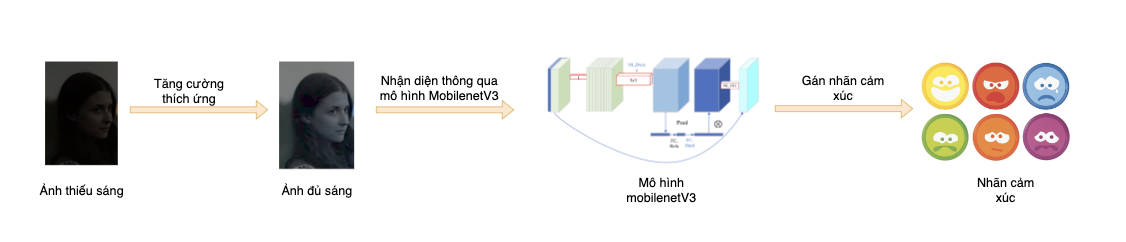
\includegraphics[width=12cm]{./img/phuong_phap_tiep_can.png} \\[0.5cm]
    \caption{Sơ đồ tổng quan quá trình nhận diện biểu cảm khuôn mặt trong điều kiện ánh sáng yếu sử dụng mô hình MobileNetV3 kết hợp tăng cường dữ liệu thích ứng.}
    \label{fig:phuong_phap_tiep_can}
\end{figure}

\begin{itemize}
    \item \textbf{Sử dụng mô hình CNN nhẹ:} MobileNetV3 được lựa chọn làm kiến trúc mạng nơ-ron nền tảng vì có dung lượng nhỏ, tốc độ suy luận nhanh và phù hợp triển khai trên thiết bị giới hạn tài nguyên. Điều này giúp đảm bảo tính khả thi trong các ứng dụng thực tế như camera an ninh, robot xã hội, hay thiết bị đeo thông minh.
    
    \item \textbf{Tăng cường dữ liệu thích ứng:} Khác với các phương pháp tăng cường dữ liệu cố định, đề tài đề xuất kỹ thuật tăng cường dựa trên mức độ sáng của từng ảnh đầu vào. Các phép biến đổi như điều chỉnh gamma, contrast stretching sẽ được áp dụng linh hoạt để mô phỏng đa dạng điều kiện ánh sáng yếu, giúp mô hình học được các đặc trưng biểu cảm một cách ổn định hơn.
\end{itemize}

Hướng tiếp cận này vừa đảm bảo hiệu quả nhận diện trong điều kiện ánh sáng khó khăn, vừa phù hợp với yêu cầu triển khai thực tế. Đề tài không chỉ có ý nghĩa trong việc nâng cao chất lượng hệ thống FER, mà còn mở ra khả năng mở rộng cho các bài toán thị giác máy tính khác trong môi trường bất lợi.

\subsection*{Câu hỏi nghiên cứu} % 2.3

Từ thực trạng và hướng tiếp cận đã trình bày, đề tài tập trung trả lời các câu hỏi nghiên cứu chính sau:

\begin{itemize}
    \item Việc áp dụng kỹ thuật tăng cường dữ liệu thích ứng theo mức độ sáng có giúp cải thiện hiệu suất nhận diện biểu cảm khuôn mặt trong điều kiện ánh sáng yếu hay không?
    
    \item Mô hình CNN nhẹ (MobileNetV3) khi kết hợp với dữ liệu đã được tăng cường thích ứng có thể đạt độ chính xác trên 70\% và đảm bảo tốc độ xử lý đủ nhanh để triển khai thực tế trên thiết bị tài nguyên thấp hay không?
\end{itemize}

\section{Mục đích và nhiệm vụ nghiên cứu} % Section 3

\subsection{Mục đích nghiên cứu}

Mục đích của đề tài là xây dựng một hệ thống nhận diện biểu cảm khuôn mặt hiệu quả trong điều kiện ánh sáng yếu, đảm bảo tính chính xác và tốc độ xử lý, đồng thời phù hợp để triển khai trên các thiết bị có giới hạn tài nguyên như camera giám sát, thiết bị di động hoặc hệ thống nhúng. Thông qua việc kết hợp mô hình CNN nhẹ (MobileNetV3) với kỹ thuật tăng cường dữ liệu thích ứng theo mức độ sáng, đề tài hướng đến giải quyết các hạn chế về hiệu suất trong môi trường ánh sáng không ổn định.

Đề tài kỳ vọng chứng minh rằng với cách tiếp cận đơn giản nhưng hợp lý, có thể đạt được độ chính xác chấp nhận được (> 70\%) trong điều kiện ánh sáng yếu mà không cần sử dụng các mô hình phức tạp hoặc chi phí cao.

\subsection{Nhiệm vụ nghiên cứu}

Để đạt được mục đích trên, đề tài cần thực hiện các nhiệm vụ chính sau:

\begin{itemize}
    \item Tìm hiểu tổng quan về các mô hình CNN nhẹ, đặc biệt là MobileNetV3, và kỹ thuật tăng cường dữ liệu liên quan đến ánh sáng yếu.
    
    \item Khảo sát và phân tích các phương pháp tăng cường dữ liệu thích ứng hiện có, từ đó đề xuất kỹ thuật phù hợp với bài toán FER.
    
    \item Tiền xử lý và xây dựng tập dữ liệu mô phỏng điều kiện ánh sáng yếu dựa trên FER-2013 hoặc các tập dữ liệu FER công khai khác.
    
    \item Thiết kế và huấn luyện mô hình MobileNetV3 kết hợp với kỹ thuật tăng cường dữ liệu thích ứng để nhận diện biểu cảm khuôn mặt.
    
    \item Đánh giá hiệu suất mô hình qua các chỉ số như Accuracy, Precision, Recall, F1-score và thời gian suy luận trên CPU.
    
    \item So sánh kết quả giữa mô hình có và không áp dụng tăng cường thích ứng để chứng minh hiệu quả của phương pháp đề xuất.
\end{itemize}

\section{Đối tượng và phạm vi nghiên cứu} % Section 4

\subsection{Đối tượng nghiên cứu}

Đối tượng nghiên cứu của đề tài là các kỹ thuật nhận diện biểu cảm khuôn mặt (Facial Expression Recognition - FER) trong điều kiện ánh sáng yếu, với trọng tâm là mô hình học sâu nhẹ (lightweight deep learning) và kỹ thuật tăng cường dữ liệu thích ứng theo mức độ sáng.

Cụ thể, đề tài tập trung vào:

\begin{itemize}
    \item Mô hình mạng nơ-ron tích chập nhẹ (MobileNetV3) trong bài toán phân loại cảm xúc khuôn mặt.
    \item Các kỹ thuật tăng cường dữ liệu ảnh thích ứng dựa trên đặc trưng ánh sáng của từng ảnh (gamma correction, contrast adjustment, histogram equalization,...).
    \item Ứng dụng các kỹ thuật trên trong điều kiện ánh sáng yếu nhằm cải thiện hiệu suất phân loại biểu cảm.
\end{itemize}

\subsection{Phạm vi nghiên cứu}

Phạm vi nghiên cứu của đề tài được giới hạn trong các nội dung sau:

\begin{itemize}
    \item Tập trung xử lý hình ảnh tĩnh (không xử lý video hoặc chuỗi hình ảnh thời gian thực).
    \item Sử dụng tập dữ liệu công khai FER-2013, với các ảnh được biến đổi để mô phỏng điều kiện ánh sáng yếu.
    \item Không sử dụng các mô hình phức tạp như GAN, Vision Transformer hoặc các kiến trúc mạng lớn có yêu cầu phần cứng cao.
    \item Hạn chế ở việc đánh giá hiệu suất mô hình dựa trên độ chính xác, thời gian suy luận và các chỉ số cơ bản (Accuracy, Precision, Recall, F1-score), không mở rộng sang các khía cạnh tâm lý học hay biểu cảm vi mô.
    \item Triển khai và đánh giá mô hình trên thiết bị CPU mô phỏng điều kiện tài nguyên thấp.
\end{itemize}

\section{Phương pháp nghiên cứu} % Section 5

Để thực hiện đề tài, nhóm áp dụng kết hợp ba nhóm phương pháp chính: phương pháp lý thuyết, phương pháp thực nghiệm và phương pháp so sánh đánh giá. Mỗi phương pháp đóng vai trò hỗ trợ từng giai đoạn cụ thể trong quá trình nghiên cứu, từ khảo sát tài liệu cho đến đánh giá hiệu quả mô hình đề xuất.

\subsection{Phương pháp lý thuyết}

\begin{itemize}
    \item Nghiên cứu tổng quan các tài liệu khoa học, công trình nghiên cứu và bài báo liên quan đến nhận diện biểu cảm khuôn mặt (FER), đặc biệt là trong điều kiện ánh sáng yếu.
    \item Tìm hiểu và phân tích các mô hình CNN nhẹ, trong đó trọng tâm là MobileNetV3 — một mô hình có khả năng triển khai thực tế trên thiết bị tài nguyên thấp.
    \item Khảo sát các kỹ thuật tăng cường dữ liệu ảnh có liên quan đến ánh sáng, như gamma correction, adaptive histogram equalization, contrast stretching... từ đó đề xuất hướng tăng cường thích ứng theo mức sáng ảnh.
\end{itemize}

\subsection{Phương pháp thực nghiệm}

\begin{itemize}
    \item Sử dụng tập dữ liệu FER-2013 làm dữ liệu huấn luyện và kiểm thử. Tiền xử lý dữ liệu bằng cách mô phỏng các điều kiện ánh sáng yếu thông qua phép biến đổi độ sáng và tương phản.
    \item Áp dụng kỹ thuật tăng cường dữ liệu thích ứng: sử dụng đặc trưng ánh sáng (ví dụ: độ sáng trung bình, histogram) của từng ảnh để áp dụng các phương pháp tăng cường phù hợp.
    \item Huấn luyện mô hình MobileNetV3 trên tập dữ liệu đã được tăng cường. Thực hiện fine-tuning mô hình để đạt được hiệu suất tốt nhất.
    \item Đánh giá mô hình theo các chỉ số chuẩn: Accuracy, Precision, Recall, F1-score và thời gian suy luận trên CPU.
\end{itemize}

\subsection{Phương pháp so sánh đánh giá}

\begin{itemize}
    \item Thực hiện so sánh giữa hai mô hình: mô hình cơ bản (không tăng cường dữ liệu thích ứng) và mô hình có áp dụng kỹ thuật tăng cường thích ứng.
    \item Phân tích kết quả định lượng (qua chỉ số) và định tính (quan sát vùng biểu cảm dễ nhận diện hơn sau tăng cường) để đánh giá hiệu quả của phương pháp đề xuất.
    \item Đánh giá mức độ cải thiện về độ chính xác và tốc độ xử lý, từ đó xác định tính khả thi của mô hình trong ứng dụng thực tế.
\end{itemize}

\section{Giả thuyết khoa học} % Section 6

Dựa trên các nghiên cứu trước và định hướng của đề tài, nhóm đưa ra các giả thuyết khoa học như sau:

\begin{itemize}
    \item \textbf{Giả thuyết 1:} Mô hình học sâu nhẹ (MobileNetV3) có thể đạt hiệu suất nhận diện biểu cảm khuôn mặt tốt trong điều kiện ánh sáng yếu nếu được huấn luyện với tập dữ liệu được tăng cường thích ứng theo mức độ sáng.
    
    \item \textbf{Giả thuyết 2:} Kỹ thuật tăng cường dữ liệu ảnh thích ứng theo đặc trưng ánh sáng đầu vào giúp cải thiện độ chính xác và khả năng khái quát hóa của mô hình so với các phương pháp tăng cường cố định truyền thống.
    
    \item \textbf{Giả thuyết 3:} Hệ thống kết hợp giữa MobileNetV3 và tăng cường dữ liệu thích ứng có thể duy trì độ chính xác trên 70\% và tốc độ suy luận dưới 0.1 giây/ảnh trên CPU, phù hợp với yêu cầu triển khai thực tế trên thiết bị giới hạn tài nguyên.
\end{itemize}

Các giả thuyết trên sẽ được kiểm chứng thông qua thực nghiệm trên tập dữ liệu FER-2013 đã xử lý, bằng các chỉ số đánh giá như Accuracy, Precision, Recall, F1-score, và thời gian xử lý.

\section{Những đóng góp mới của đề tài} % Section 7

Đề tài không chỉ tiếp cận bài toán nhận diện biểu cảm khuôn mặt theo hướng tối ưu tài nguyên mà còn đề xuất cách tiếp cận hiệu quả trong điều kiện ánh sáng yếu – một thách thức phổ biến trong ứng dụng thực tiễn. Những đóng góp mới của đề tài bao gồm:

\begin{itemize}
    \item \textbf{Đề xuất kỹ thuật tăng cường dữ liệu thích ứng theo mức độ sáng:} Khác với các phương pháp tăng cường cố định truyền thống, nhóm đã thiết kế cơ chế tăng cường ảnh linh hoạt dựa trên đặc trưng ánh sáng đầu vào (trung bình độ sáng, histogram, v.v.). Kỹ thuật này giúp cải thiện khả năng học và tổng quát hóa của mô hình trong các tình huống ánh sáng không đồng đều.

    \item \textbf{Ứng dụng mô hình CNN nhẹ (MobileNetV3) trong điều kiện ánh sáng yếu:} Đề tài chứng minh rằng, với phương pháp xử lý dữ liệu phù hợp, các mô hình CNN nhẹ hoàn toàn có thể đạt hiệu suất tốt mà vẫn đảm bảo tốc độ suy luận nhanh – mở ra khả năng triển khai thực tế trong các hệ thống giám sát, thiết bị IoT, hoặc môi trường có giới hạn tài nguyên.

    \item \textbf{Tạo tập dữ liệu ánh sáng yếu có tính đại diện cao:} Nhóm đã xây dựng tập dữ liệu mô phỏng ánh sáng yếu từ FER-2013 với nhiều cấp độ sáng khác nhau, phục vụ cho huấn luyện và đánh giá mô hình. Đây có thể là tài nguyên tham khảo hữu ích cho các nghiên cứu liên quan trong tương lai.

    \item \textbf{Thực nghiệm so sánh có định hướng rõ ràng:} Đề tài không chỉ triển khai mô hình mà còn thực hiện đánh giá định lượng giữa các phương pháp có và không có tăng cường thích ứng, giúp làm rõ hiệu quả thực sự của hướng tiếp cận đề xuất.

\end{itemize}

Những đóng góp trên, tuy ở mức ứng dụng, nhưng có ý nghĩa thực tiễn cao và có thể trở thành tiền đề cho các nghiên cứu chuyên sâu hơn trong lĩnh vực nhận diện biểu cảm trong điều kiện ánh sáng không lý tưởng.

\section{Dự kiến kế hoạch nghiên cứu} % Section 8

Kế hoạch thực hiện đề tài được chia thành các giai đoạn rõ ràng, từ nghiên cứu lý thuyết, thu thập dữ liệu, đến thực nghiệm và viết báo cáo. Nhóm dự kiến hoàn thành trong thời gian 8 tuần như sau:

\begin{center}
\renewcommand{\arraystretch}{1.5}
\begin{tabular}{|c|p{8cm}|c|}
    \hline
    \textbf{STT} & \centering \textbf{Nội dung công việc} & \textbf{Thời gian} \\ \hline
    1 & Tìm hiểu tổng quan về nhận diện biểu cảm khuôn mặt, điều kiện ánh sáng yếu và các mô hình CNN nhẹ & Tuần 1 \\ \hline
    2 & Khảo sát kỹ thuật tăng cường dữ liệu và đề xuất phương pháp tăng cường thích ứng theo ánh sáng ảnh & Tuần 2 \\ \hline
    3 & Tiền xử lý dữ liệu FER-2013 và xây dựng tập dữ liệu mô phỏng điều kiện ánh sáng yếu & Tuần 3 \\ \hline
    4 & Huấn luyện mô hình MobileNetV3 cơ bản và tinh chỉnh tham số & Tuần 4 \\ \hline
    5 & Tích hợp kỹ thuật tăng cường thích ứng vào pipeline huấn luyện & Tuần 5 \\ \hline
    6 & Đánh giá mô hình: so sánh với mô hình không tăng cường; phân tích kết quả qua các chỉ số & Tuần 6 \\ \hline
    7 & Viết báo cáo, chuẩn bị biểu đồ, bảng số liệu, hình ảnh minh họa & Tuần 7 \\ \hline
    8 & Rà soát, chỉnh sửa báo cáo, hoàn thiện đề cương và chuẩn bị bảo vệ & Tuần 8 \\ \hline
\end{tabular}
\end{center}

Kế hoạch có thể được điều chỉnh linh hoạt tùy theo tiến độ thực tế, tuy nhiên nhóm sẽ đảm bảo hoàn thành đúng hạn và chất lượng tốt nhất.

\section{Dự kiến nội dung của luận văn} % Section 9

Luận văn dự kiến được chia thành 5 chương chính như sau:

\begin{itemize}
    \item \textbf{Chương 1 – Giới thiệu đề tài}  
    \begin{itemize}
        \item Bối cảnh, lý do chọn đề tài  
        \item Mục tiêu, đối tượng, phạm vi nghiên cứu  
        \item Ý nghĩa khoa học và thực tiễn  
    \end{itemize}

    \item \textbf{Chương 2 – Cơ sở lý thuyết và tổng quan nghiên cứu}  
    \begin{itemize}
        \item Các kỹ thuật nhận diện biểu cảm khuôn mặt  
        \item Kiến trúc CNN nhẹ (đặc biệt là MobileNetV3)  
        \item Kỹ thuật tăng cường dữ liệu và các công trình liên quan  
    \end{itemize}

    \item \textbf{Chương 3 – Phương pháp đề xuất}  
    \begin{itemize}
        \item Chi tiết kỹ thuật tăng cường dữ liệu thích ứng  
        \item Ứng dụng trên tập dữ liệu FER-2013  
        \item Tích hợp với mô hình MobileNetV3  
    \end{itemize}

    \item \textbf{Chương 4 – Thực nghiệm và đánh giá}  
    \begin{itemize}
        \item Thiết lập huấn luyện và tham số mô hình  
        \item Đánh giá theo các chỉ số: Accuracy, F1-score, v.v.  
        \item So sánh mô hình có và không có tăng cường thích ứng  
    \end{itemize}

    \item \textbf{Chương 5 – Kết luận và hướng phát triển}  
    \begin{itemize}
        \item Tổng kết nội dung đã thực hiện  
        \item Đánh giá ưu, nhược điểm  
        \item Đề xuất hướng phát triển trong tương lai  
    \end{itemize}
\end{itemize}

\section{Danh mục tài liệu tham khảo} % Section 10

\endgroup
\end{document}